\section{Introduction}


\subsection{The IR camera}
Electromagnetic radiation of wavelengths between $700$ nanometer to $1$ millimeter comprise what is usually referred to as \textit{infrared light}. Much like the normal camera is able to detect and display variations of visible light (having wavelength spectrum just below infrared light), infrared cameras produce pictures colored according to the variations in infrared radiation  (IR) of a scene. Since infrared emission from an object is closely related to its temperature, an IR camera essentially produces a heat map to the eye, coloring parts of a scene relative to temperature. Many infrared cameras are also able to accurately estimate the temperature of an object in addition to depicting it.

\begin{figure}[h]
\begin{center}
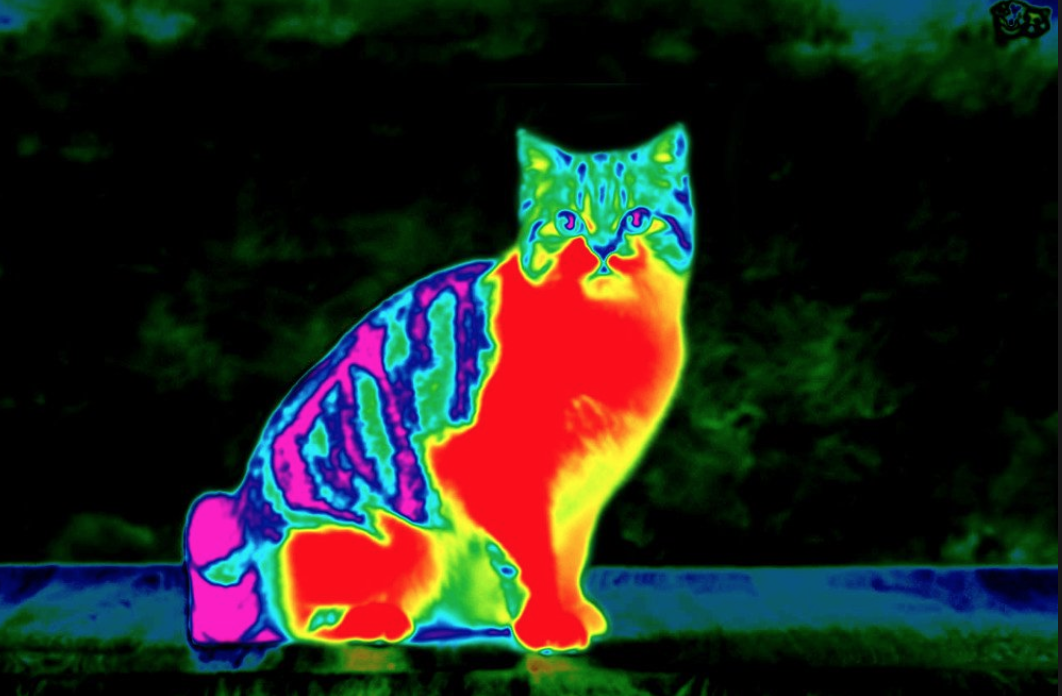
\includegraphics[height=5cm]{gfx/cat.png}
\caption{Infrared picture of a cat sitting on a table during night. The warmblooded cat is clearly distinguished from its cold surrounding, making the cat visible to the IR camera although not visible to the eye. \gm{CITE THE SOURCE OF THIS FIGURE!} }
\end{center}
\end{figure}

Infrared cameras are used widely within industrial and military
applications, enabling or enhancing tasks such as dark vision, heat
leakage detection, moisture detection, chemical spill leakage
detection and firefighting. An overview about different devices
together with a catalog can be found in~\cite{flir_handbook}. There
exist mainly two types of techniques for infrared cameras: thermal
detectors and quantum detectors. We will here focus solely on a
special type of thermal detectors, using as its central device a so
called \textit{bolometer}. The bolometer consists of a plate (pixel)
made of metal or semiconductor material, an example being a mixture of
silicon nitride and vanadium oxide. This plate is mounted on a
substrate via two supporting legs, and connected to a voltage
source. Incoming infrared radiation is focused via a lens to the
plate, causing it to be heated, which in turn alters its
resistance. This change in resistance can be measured through the
input voltage and resulting current, resulting in a signal that is a
function of the strength of the incoming infrared radiation and hence
the temperature of a partial scene.

\begin{figure}[h]
\begin{center}
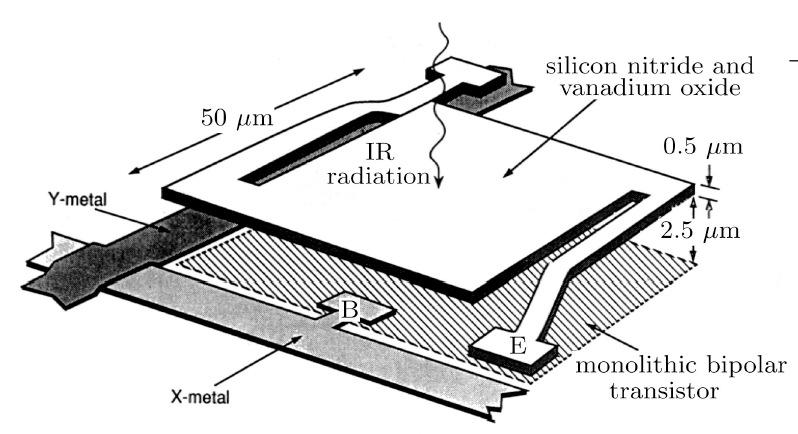
\includegraphics[height=5cm]{gfx/pixel1.png}
\caption{ \gm{CITE THE SOURCE OF THIS FIGURE!} }
\end{center}
\end{figure}

\subsection{Project description}
The project aims to establish a mathematical relationship between the temperature of an object and the resulting bolometer signal.
%As starting point for the analysis, we use the modeling framework from \cite{xiu2010research}. The signal here is described through the differential equation:

%\begin{align}
%C_{\rm int}\frac{d v_s}{dt}&=\frac{V_0}{R(T_s)}-\frac{V_b(t)}{R(T(t))} \\
%\end{align}

%Here $v_s$ is the output signal, $V_0$ is a reference voltage, $R$ is the resistance of the pixel as a function of temperature, $V_{b}$ is the applied voltage through the pixel as a function of time, $T$ is the temperature of the pixel as a function of time, and $T_s$ is the constant temperature of the substrate. The temperature as a function of time is described through the differential equation:

Roughly speaking, the bolometer is a resistor whose resistance depends on the temperature.
The temperature of the bolometer as a function of the time (and the incoming IR radiation) is described by the following differential equation
\begin{align} \label{eq:heat_balance_equation}
 C\frac{dT}{dt}&=\frac{V_b(t)^2}{R(T)}+\varepsilon(P_t+P_s -2A_s \sigma T^4)-G_{leg}(T-T_s) \\
 T(0)&=T_s	\nonumber
\end{align}
Here $V_b(t)$ is the input voltage, $\varepsilon_e$ is the material specific emissivity of the pixel, $P_t$ is the radiation power from the scene, $P_s$ is the radiation power from the substrate, $2A_s$ is the surface area of the pixel, $\sigma$ is the Boltzmann constant, G is thermal conductivity of the supporting legs. The term $V_b(t)^2/R(T)$ is the power resulting from applying the voltage over the pixel, and $2A_s \sigma T^4$ represents the radiation power emitted from a black body according to Stefan-Boltzmann's law. The latter also relates $P_t$ to the temperature $\tilde T$ of a scene object as $P_t = A_s \sigma (T_0+\tilde T)^4$.
The temperature dependent resistance of the bolometer $R(T)$ is estimated by measuring the voltage across certain specific components of the circuit where the bolometer is located. More precisely, the output signal is a voltage that can be used to retrieve $R(T)$ and sequentially compute the temperature of the pixel. An explicit description of the output signal is given in Section~\ref{sec:model_disc}.

%By solving the ODE's numerically, we can get the output signal $v_s$ as a deterministic function of $T_o$. In reality however, the output signal $v_s$ is noisy. The project aims to incorporate noise into the model in a manner consistent with data and experience. A good model of the noisy signal might for example enable an efficient filtering that reduces noise.

In reality however, the output signal is noisy. The project aims to incorporate noise into the model in a manner consistent with data and experience. A good model of the noisy signal might for example enable an efficient filtering that reduces noise. The project's aim is to investigate how a noisy input signal effects the output signal.

More precisely in this project we
\begin{itemize}
 \item simulate the read-out signal of the bolometer by solving the differential equations modeling the problem,
 \item reproduce numerical simulations that fits with empirical experiments,
 \item model and analyze the noise in the differential equations,
 \item reproduce numerical simulations (with noise) that fits with empirical experiments.
\end{itemize}
